\section*{Общая характеристика работы}

\newcommand{\actuality}{\underline{\textbf{\actualityTXT}}}
\newcommand{\progress}{\underline{\textbf{\progressTXT}}}
\newcommand{\actualityandprogress}{\underline{\textbf{\actualityandprogressTXT}}}
\newcommand{\aim}{\underline{{\textbf\aimTXT}}}
\newcommand{\tasks}{\underline{\textbf{\tasksTXT}}}
\newcommand{\novelty}{\underline{\textbf{\noveltyTXT}}}
\newcommand{\influence}{\underline{\textbf{\influenceTXT}}}
\newcommand{\methods}{\underline{\textbf{\methodsTXT}}}
\newcommand{\defpositions}{\underline{\textbf{\defpositionsTXT}}}
\newcommand{\reliability}{\underline{\textbf{\reliabilityTXT}}}
\newcommand{\probation}{\underline{\textbf{\probationTXT}}}
\newcommand{\contribution}{\underline{\textbf{\contributionTXT}}}
\newcommand{\publications}{\underline{\textbf{\publicationsTXT}}}

{\actualityandprogress}. Методы восстановления измерений в задаче компьютерной томографии можно разделить на интегральные и алгебраические. К интегральным относится метод светки и обратной проекции....

{\aim} ~данной работы являются разработка метода реконструкции, позволяющего учесть присутствие в объекте сильнопоглощающих включений, а так же метода численной интерпретации результатов измерений многокомпонентных объектов.

Для достижения поставленной цели были решены следующие {\tasks}:
\begin{enumerate}
  \item построен асимптотически быстрый алгебраический метод реконструкции, основанный на применении быстрого преобразования Хафа.
  \item доказана сходимость построеного алгебраического метода реконструкции, за счет полученного математического выражения градиента быстрого преобразования Хафа.
  \item построен алгоритм реконструкции для объектов, содержащих сильнопоглощающие включения.
  \item построен алгоритм реконструкции, учитывающий покомпонентное ослабление полихроматического спектра.
\end{enumerate}

{\novelty}
\begin{enumerate}
  \item Впервые для реконструкции томографических измерений было применено быстрое преобразование Хафа.
  \item Впервые получено выражение для производной быстрого преобразования Хафа, а так же алгоритм его эффективного вычисления.
  \item Построен алгоритм реконструкции, учитывающий вклад сильно поглощающих включений с помощью оригинальной модели ограничений-неравенств.
  \item Предложена схема обработки данных полихроматического зондирования, при которой восстанавливаются реальные физические концентрации элементов.
\end{enumerate}

{\influence} ~Результаты, полученные в диссертационной работе, используются для обработки данных лабораторных исследований. Построенные алгоритмы лягут в основу программного обеспечения новых моделей промышленных томографов.

Полученное в работе выражение для градиента быстрого преобразования Хафа имеет общетеоретическое значение и уже применяется в области машинного обучения для обратного распространения ошибки в нейронных сетях глубокого обучения через слой БПХ.

{\methods}
Для решения задач реконструкции томографических измерений используются методы теории условной и безусловной оптимизации: градиентные методы оптимизации, квадратичное программирование, регуляризация.
Для ускорения итерации алгебраического метода используются алгоритмы обработки изображений в виде быстрого преобразования Хафа.


{\defpositions}
\begin{enumerate}
  \item Предложен эффективный вычислительный метод решения задачи томографической реконструкции FHT-SIRT, основанный на алгебраическом подходе, который позволяет снизить асимптотическую оценку сложности вычисления итерации с $O(n^3)$ до $O(n^2~\log n)$, что подтвержается численными экспериментами и замерами времени работы программной реализации алгоритма.
  \item Проведено математическое обоснование сходимости предложенного метода.
  \item Предложен метод реконструкции на основе квадратичного программирования, который позволяет уменьшить артефакты на восстановленном изображении, вызванные наличием сильно поглощающих областей в зондируемом объекте.
  \item Предложен алгебраический метод реконструкции для случая полихроматического зондирования, который решает оптимизационную задачу реконструкции относительно линейной комбинации концентраций с ограничениями-неравенствами на их область значений.
\end{enumerate}


{\reliability} полученных результатов обеспечивается модельными экспериментами и численными симуляциями, а так же экспериментами с восстановлением реально измеренных в лабораторных условиях образцов.\ Результаты находятся в соответствии с результатами, полученными другими авторами.


{\probation}
Основные результаты работы докладывались~на: конферециях 
35-я конференция молодых ученых и специалистов «Информационные технологии и системы» (2012, 19 - 25 августа, Петрозаводск, Россия),
11th Biennal Conference on High Resolution X-Ray Diffraction and Imaging (XTOP 2012, St. Petersburg, Russia), 
29th European Conference on Modelling and Simulation (ECMS 2015, Albena, Bulgaria),
Eighth International Conference on Machine Vision (ICMV 2015, Barcelona, Spain),
на общефизическом семинаре ИПТМ РАН (октябрь 2016).

{\contribution} Все результаты диссертации, вынесенные на защиту, получены автором самостоятельно.
Автором самостоятельно реализованы методы восстановления FHT-SIRT из первой главы, барьерных функций из второй, метод взвешанных невязок из третьей, проведены численные экспериметны по обработке реальных и модельных данных.
Постановка задач и обсуждение результатов проводились совместно с научным руководителем.
Генерация модельных данных для экспериментов в полихроматике проводилась аспирантом факультета КН НИУ ВШЭ Ингачевой А.~С. 
Программная имплементация метода мягких ограничений, использованная для сравнения с методом барьерных функций во второй главе, принадлежит Соколову В.~В.
Измерения для экспериментов по восстановлению зуба со свинцовым включением производились на лабоработном источнике ИК РАН в лаборатории рефлектометрии и малоуглового рассеяния.
Многие аспекты исследований в разное время обсуждались с Чукалиной М.~В., Николаевым Д.~П., Бузмаковым А.~В., Ингачевой А.~С., Соколовым В.~В.


\ifthenelse{\equal{\thebibliosel}{0}}{% Встроенная реализация с загрузкой файла через движок bibtex8
    \publications\ Основные результаты по теме диссертации изложены в 11 печатных изданиях, 
    3 из которых изданы в журналах, рекомендованных ВАК, 
    6 "--- в тезисах докладов.%
}{% Реализация пакетом biblatex через движок biber
%Сделана отдельная секция, чтобы не отображались в списке цитированных материалов
  \begin{refsection}%
    \printbibliography[heading=countauthorvak, env=countauthorvak, keyword=biblioauthorvak, section=1]%
    \printbibliography[heading=countauthornotvak, env=countauthornotvak, keyword=biblioauthornotvak, section=1]%
    \printbibliography[heading=countauthorconf, env=countauthorconf, keyword=biblioauthorconf, section=1]%
    \printbibliography[heading=countauthor, env=countauthor, keyword=biblioauthor, section=1]%

    \publications\ Основные результаты по теме диссертации изложены в \arabic{citeauthor} печатных изданиях \nocite{PruBuzNik13, Prun2013Crys, Vestnik2016, Prun2013AutomAndRemCont, buz_jac_2015, chukalina2014xray}, 
    \arabic{citeauthorvak} из которых изданы в журналах, рекомендованных ВАК %\nocite{PruBuzNik13, Prun2013Crys, Vestnik2016}, 
    \arabic{citeauthorconf} "--- в тезисах докладов \nocite{itas2015Prun,itas2015Ingacheva,ecms2015Chukalina, icmv2015Chukalina, embc2013Buzmakov, nikolaevfast}.
  \end{refsection}
} % Характеристика работы по структуре во введении и в автореферате не отличается (ГОСТ Р 7.0.11, пункты 5.3.1 и 9.2.1), потому её загружаем из одного и того же внешнего файла, предварительно задав форму выделения некоторым параметрам

%Диссертационная работа была выполнена при поддержке грантов ...

%\underline{\textbf{Объем и структура работы.}} Диссертация состоит из~введения, четырех глав, заключения и~приложения. Полный объем диссертации \textbf{ХХХ}~страниц текста с~\textbf{ХХ}~рисунками и~5~таблицами. Список литературы содержит \textbf{ХХX}~наименование.

%\newpage
\section*{Содержание работы}
Во \underline{\textbf{введении}} приводится общая характеристика работы, 
обоснована актуальность, цель диссертации, научная новизна, показана теоретическая и практическая значимость исследований,
проведённых в рамках данной диссертационной работы, представлены методы исследования, указана степень достоверности и апробация результатов.

В \underline{\textbf{первой главе}} формулируется математическая постановка задачи, приводится обзор актуальной научной литературе по теме.

Формулируется модель формирования измерений с параллельным пучком при зондировании монохроматическим излучением. 
Задача восстановления томографических измерений ставится как обращение преобразования Радона 
\begin{equation}\notag
  p(\varphi, \xi) = \ln \left (\frac{I_0}{I(\varphi, \xi)} \right) = 
 \iint \! \mathrm d x \mathrm d y f(x,y)\delta(x\cos\varphi + y\sin\varphi - \xi).
\end{equation}
Задача состоит в восстановлении функции ослабления рентгеновского излучения $f(x,y)$ по набору логарифмированных нормированных проекций под разными углами $p(\varphi, \xi)$.

Для решения этой задачи существует две основных группы методов: интегральные и алгебраические.
Основой первой группы методов является алгоритм свертки и обратной проекции, или FBP. 
Этот алгоритм основан на обращении фурье-образов измеренных проекций целевой функции.
Будучи основанным на дискретном преобразовании фурье, алгоритм реконструкции имеет низкую вычислительную сложность $O(n^2 \log n)$, однако зачастую в восстановлении этим методом присутствуют характерные артефакты восстановления.
Обычно их подавляют с помощью фильтрации на этапе пост-обработки.

Другая группа методов --- алгебраические, использует численные методы решения СЛАУ в дискретном приближении оператора преобразования Радона.
Это приближение называется преобразованием Хафа, и может быть выражено в виде матрицы весов $W \in Mat\left(n^2 \times n ~ n_\varphi\right)$.
Полученную систему $p = Wf$ решают итерационными методами.
Например, классический алгоритм ART использует метод Карчмарша, метод SIRT --- градиентный спуск, а метод SART --- частичный градиентный спуск по тем координатам градиента, которые соответствуют лучам, направленным под одним углом.
Алгебраические методы являются более вычислительно тяжелыми, в то время как позволяют добиться лучшего качества восстановления, чем интегральные.
В частности, алгебраические методы позволяют учесть специфику задачи и причину возникновения конкретных артефактов, учтя это во время восстановления, а не на этапе постобработки.

К таким артефактам можно отнести артефакты вызванные наличием сильнопоглощающих включений.
Столкнуться с такими артефактами можно, например, при медицинском сканировании пациента с металлическими коронками в зубах или костными протезами.
Причиной таких артефактов является недостаточное количество фотонов, проходящих через такие включения.
Для борьбы с ними используют как аппаратные так и праграммные методы.
Примерами аппаратных могут быть адаптивное расширение детектирующей ячейки в местах дефицита фотонов, зондирование несколькими энергиями.
Чтобы бороться с данным эффектом программно, испоьлзуют статистические методы, например метод максимального правдоподобия, чтобы исправить синограмму в местах некорректно интерпретируемых данных.

Одна из причин возникновения артефактов, в том числе и вызыванных наличием сильнопоглощающих включений, является отсутствие учета полихроматичности спектра источника в модели формирования томографических измерений.
При этом применяют как изменения в экспериментальной схеме --- зондирование разными спектрами или применение монохроматоров, так и модифицирование методов восстановления.


Во \underline{\textbf{второй главе}} предложен и обсуждается асимптотически быстрый алгоритм SART, основанный на реализации быстрого преобразования Хафа (БПХ).
Алгоритм решает задачу восстановления для случая зондирования монохроматическим параллельным излучением.
Требуемое доказательство асимптотической оценки сложности алгоритма представлено.
Численная реализация алгоритма проиллюстрирована результатами реконструкции модельного изображения размером 256 $\times$ 256 по полному набору 1021 углов БПХ и по разреженным синограммам, имеющим до 11 раз меньшее число проекционных углов.

Обычно итерация алгебраического метода выглядит как шаг в направлении антиградиента минимизируемого функционала ошибки:
\begin{equation}\notag
  \Delta \textbf f = \sum_\varphi {{W^\varphi}^{\mathrm T}(\textbf p - W\textbf f) } = W^{\mathrm T}(\textbf p - W \textbf f).
\end{equation}
где $W$ это оператор преобразования Хафа или томографической проекции.
  
Для асимптотического ускорения итерации алгебраического метода предлагается использовать приближенное вычисление преобразования Радона для конечного набора углов (преобразование Хафа), основанное на диадических паттернах --- быстрое преобразование Хафа.
Общая схема алгоритма состоит в следующем: сначала данные эксперимента трансформируются, чтобы реальные углы и смещения измерительной схемы соответствовали правильным координатам изображения, полученного после БПХ.
\todo{вставить формулы и картинки с четвертями БПХ}
После этого происходит итеративная процедура, вычисляющая прямую проекцию от текущей гипотезы о восстанавливаемом объекте, вычислении невязки, вычисления градиента невязки и обновления гипотезы.
Замена поворота в модели прямой проекции производится очевидным образом.
При вычислении невязки нужно учитывать отсутствующие измерения в реальных экспериментальных данных: например, если число проекционных углов составляет $n_\varphi$, то в хафовских координатах такая картина будет иметь нули по $4 * n - 3 - n_\varphi$ угловым отсчетам.

Эффективная реализация обратной проекции (вычисления градиента невязки) с помощью БПХ требует детального описания.
БПХ-изображение можно разделить на 4 части по направлениям линий проекции: вертикальные-левые, вертикальные-правые, горизонтальные-левые и горизонтальные-правые.
Соответственно, матрица проекции $W$ тоже разделяется на 4 независимые части по строкам.
Для каждой четверти преобразования Хафа выполняются аналогичные действия.

Показано, что можно использовать метод FHT-SIRT для восстановления томографии.
При этом одна итерация зависит только от четверти проекционных углов, поэтому возможно использовать модификацию FHT-SART чтобы сделать итерационный процесс ближе к методу SART, который обладает лучшей сходимостью.
Использование FHT-SIRT позволяет снизить асимптотическую сложность одной итерации метода с $O(n^2 * n_\varphi) \approx O(n^3)$ до $O(n^2 \log n)$.
При восстановлении данных реальных экспериментов количество и значения проекционных углов не соответствуют полностью заполненному FHT-преобразованию. 
Исследовано влияние степени разрежения на качество сходимости \ref{fig:conv_all} a).

\begin{figure}
\centering
\begin{tabular}{@{}c@{}c}
    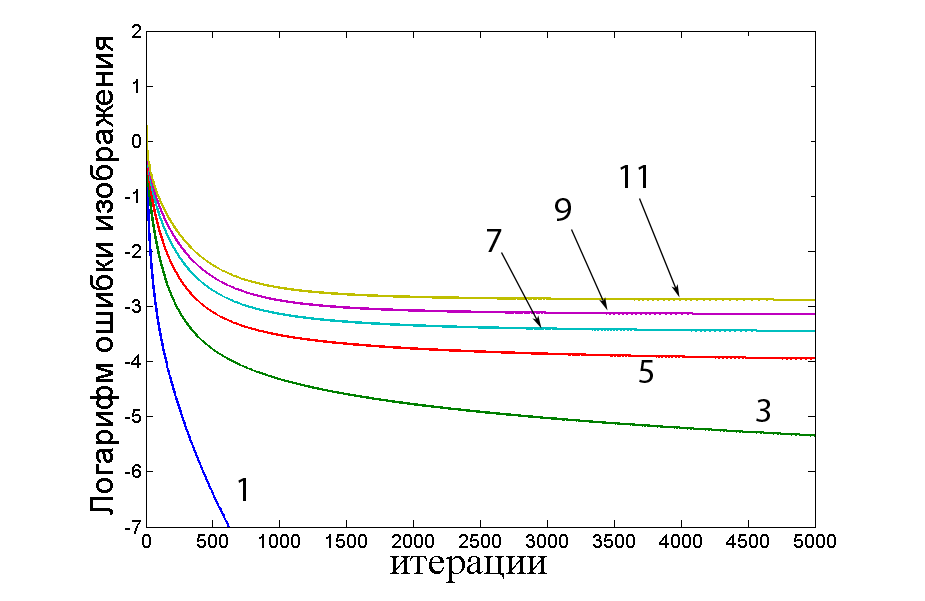
\includegraphics[width=0.45\textwidth]{Dissertation/images/part1_img/raw}
&
    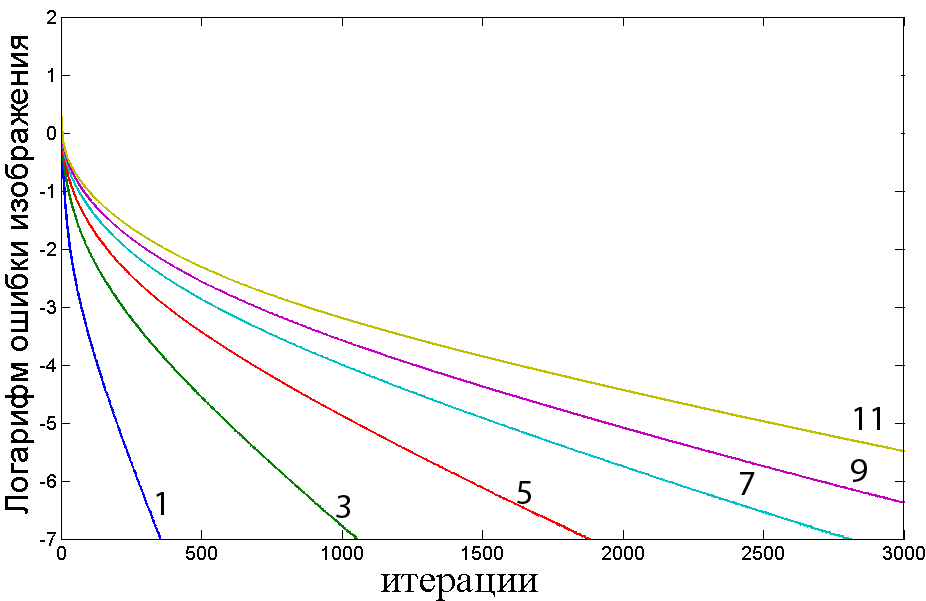
\includegraphics[width=0.45\textwidth]{Dissertation/images/part1_img/medk}
\\
   \small a) & \small b)
\end{tabular}
  \caption{Зависимость среднеквадратичной ошибки изображения от числа итераций.}
Число рядом с кривой соответствует степени разрежения. а --- Без регуляризации, б --- Медианная регуляризация.
\label{fig:conv_all}
\end{figure}

Кроме того, при переводе синограммы из измеренных координат $\rho, \varphi$ в координаты пространства БПХ, нужно учесть изменение ширины БПХ-луча, то есть отнормировать соответствующую строчку синограммы по ширине и интенсивности.

Для лучшей сходимости метода исследуются возможные регуляризации при применении метода FHT-SART.
Исследуются регуляризация с применением медианного, билатерального фильтров, а так же регуляризация по Тихонову.
Приводятся результаты восстановления с применением указанных видов регуляризации.
В частности, сравнение сырого восстановления с медианной регуляризацией, приведено на рис. \ref{fig:conv_all}.


В \underline{\textbf{третьей главе}} предложена модель формирования измерений при наличии в объекте сильнопоглощающих включений.
При прохождении через такие включения, например, металлический протез в зубе, большая часть зондирующего излучения поглощается.
В результате количество фотонов, доходящих до детектора недостаточно для активации его пикселя.
При измерении с таких пикселей считывается значение 0, хотя, на самом деле, можно лишь сказать, что значение, считанное с этих пикселей находится где-то в интервале $[0, \delta_min)$, где $\delta_min$ --- минимальный порог срабатывания детектора, или уровень шума.

В результате задачу восстановления томографии в алгебраическом подходе можно модифицировать, введя ограничения типа неравенства для измерений, значение которых 0.
С учетом перехода к логарифмам измеренной интенсивности, 

\begin{equation} \notag
  \label{eq:quadprog_ineq}
  \begin{cases}
  \Norm{P^{\textup{изм.}} - P(\mu)} \rightarrow \min_{\mu} & w.r.t \\
  \sum_i \mu_{i} \omega_{ij} = P_j, & \mbox{если} P^{\textup{изм.}}_j < \mbox{порог} \\
  \sum_i \mu_{i} \omega_{ij} > \mbox{порог}, & \mbox{если} P^{\textup{изм.}}_j = \mbox{порог}
  \end{cases}
\end{equation}

Для решения этой минимизационной задачи предложено применить метод квадратичного программирования.



Производятся исследования метода мягких ограничений на основе данных реальных экспериментальных измерений.

В \underline{\textbf{четвертой главе}} предложен алгебраический метод для восстановления томографических измерений при зондировании полихоматическим илучением.

В \underline{\textbf{заключении}} приведены основные результаты работы, которые заключаются в следующем:
%% Согласно ГОСТ Р 7.0.11-2011:
%% 5.3.3 В заключении диссертации излагают итоги выполненного исследования, рекомендации, перспективы дальнейшей разработки темы.
%% 9.2.3 В заключении автореферата диссертации излагают итоги данного исследования, рекомендации и перспективы дальнейшей разработки темы.
\begin{enumerate}
  \item Получено аналитическое выражение для операции транспонированного быстрого преобразования Хафа. Доказана теорема о симметричности четверти БПХ, отвечающей одной группе ориентаций лучей. Получен метод вычислительно эффективного вычисления транспонированного преобразования.
  \item Построен вычислительно эффективный алгебраический метод восстановления измерений компьютерной томографии на основе БПХ. Произведена адаптация метода для работы с данными реальных измерений. Изучены свойства пространства БПХ, влияние различной регуляризации на процесс восстановления.
  \item Построен метод восстановления рентгеновской томографии методом квадратичного программирования для объектов, содержащих сильнопоглощающие включения. На реальных экспериментальных измерениях проведено исследование метода мягких ограничений \todo{и сравнение с методом квадратичного программирования}
  \item Построен алгебраический алгоритм восстановления томографии в задаче зондирования полихроматическим излучением, основанный на вычиследнии взвешанных невязок по каждому из элементов, входящих в состав исследуемого образца. Предложены варианты регуляризации для востановления в полихроматической моде. \todo{описать, какой получен результат}
\end{enumerate}



\begin{comment}
%\newpage
При использовании пакета \verb!biblatex! список публикаций автора по теме
диссертации формируется в разделе <<\publications>>\ файла
\verb!../common/characteristic.tex!  при помощи команды \verb!\nocite! 
\end{comment}

\newpage
\ifdefmacro{\microtypesetup}{\microtypesetup{protrusion=false}}{} % не рекомендуется применять пакет микротипографики к автоматически генерируемому списку литературы
\ifnumequal{\value{bibliosel}}{0}{% Встроенная реализация с загрузкой файла через движок bibtex8
  \renewcommand{\bibname}{\large \authorbibtitle}
  \nocite{*}
  \insertbiblioauthor           % Подключаем Bib-базы
  %\insertbiblioother   % !!! bibtex не умеет работать с несколькими библиографиями !!!
}{% Реализация пакетом biblatex через движок biber
  \ifnumgreater{\value{usefootcite}}{0}{
%  \nocite{*} % Невидимая цитата всех работ, позволит вывести все работы автора
  \insertbiblioauthorcited      % Вывод процитированных в автореферате работ автора
  }{
  \insertbiblioauthor           % Вывод всех работ автора
%  \insertbiblioauthorgrouped    % Вывод всех работ автора, сгруппированных по источникам
%  \insertbiblioauthorimportant  % Вывод наиболее значимых работ автора (определяется в файле characteristic во второй section)
  \insertbiblioother            % Вывод списка литературы, на которую ссылались в тексте автореферата
  }
}
\ifdefmacro{\microtypesetup}{\microtypesetup{protrusion=true}}{}

